\section{Juegos de estrategia por turnos}

También conocidos como \textit{turn-based strategy} (TBS), son juegos donde el tiempo de juego no transcurre de forma continua, si no que se divide en partes bien definidas llamadas turnos. En un turno, un jugador dispone de un periodo de análisis antes de realizar una acción, lo cual realiza un salto de turno al siguiente jugador. Cuando todos los jugadores han terminado su turno, se comienza una nueva ronda. \\

Existen varios géneros dentro de la estrategia por turnos: 

\begin{itemize}
	\item \textbf{Juegos clásicos de tablero}: Son los primeros juegos de este tipo, padres del resto de géneros. La idea es controlar la acción del propio juego mediante turnos. En este género tenemos como ejemplos el ajedrez, el Go o el Revesi.
	\item \textbf{TBS and RTT} (Estrategia por turnos y táctica en tiempo real): Añade un componente en tiempo real al permitir que en cada turno se generen batallas en tiempo real contra los oponentes. Un ejemplo de este género es la saga de videojuegos Total War.
	\item \textbf{Man-to-man}: Se basa en el uso de unidades muy pequeñas, en donde controlamos cada uno de los individuos de nuestra partida. En esta categoría está la saga de videojuegos XCOM.
	\item \textbf{TRPG} (RPG táctico): También conocidos en Japón como Simulation RPG (SRPG), se basan en incorporar elementos de estrategia por turnos al combate clásico de los RPG. En la parte de tablero, un ejemplo clásico es Dragones y Mazmorras (\textit{Dungeons \& Dragons}), mientras que en el caso de los videojuegos, los más conocidos son Darkest Dungeon, algunas entregas de Megami Tensei como Shin Megami Tensei y Persona, la saga Disgaea o Fire Emblem.
	\item \textbf{4X}: Llamado así por la idea principal del género (\textit{eXplore, eXpand, eXploit and eXterminate}, en castellano ``Explora, expande, explota y extermina"). Se basan en el control de un imperio, profundizando en el desarrollo económico, tecnológico y militar, con la idea final de que crear a largo tiempo un imperio sostenible. Existe una profunda complejidad debido a la cantidad de elementos que hay que tener en cuenta. Un ejemplo en tablero de este género es Risk, mientras que en videojuegos destaca la saga Master of Orion y Sid Meier's: Civilization [ver sección \ref{subsec:civ}].
\end{itemize}

\subsection{Sid Meier's: Civilization}\label{subsec:civ}

Como ya comenté, Civilization\footnote{https://civilization.com} es un videojuego de estrategia por turnos que cae dentro del género X4, lanzado por primera ver en 1991 por el programador y diseñador Sid Meier. El objetivo del juego es construir una civilización y avanzarla desde la prehistoria y hasta un futuro cercano. En cada turno, el jugador puede mover unidades por el mapa, construir o mejorar ciudades y unidades, y realizar negociaciones con el resto de jugadores. Una vez se realiza una ronda, el juego avanza unos años en la historia. Actualmente existen seis títulos principales (a la hora de escribir esta memoria el último juego lanzado fue Civilization VI en 2016) y varios spin-off que se centran en potenciar distintos aspectos de los títulos principales. \\

Al empezar la partida, el jugador se encuentra en un mapa basado en casillas generado proceduralmente, el cual contiene distintos biomas (praderas, desierto, montañas, ríos, lagos, etc...) con una serie de recursos (vino, caballos, trigo, fuel, carbón, etc...). La posición inicial normalmente es aleatoria, y el jugador puede controlar con una serie de colonos. En el resto del mapa cercano a los colonos, existe una niebla de guerra para evitar que el jugador pueda ver que hay cerca de el. \\

Si el jugador decide fundar una ciudad con los colonos, esta empieza a general recursos que pueden ser los propios del mapa que hay en las casillas cercanas a la ciudad o simplemente mano de obra, cultura, ciencia o dinero. La cantidad de recursos que se puede generar en una ciudad se basa en como de grande es esta. Con estos recursos, se puede producir nuevas unidades como colonos, guerreros, distintos elementos de guerra como barcos, aviones y maquinaria pesada, o unidades con las que mantener comercio con otras civilizaciones. \\

Con la ciencia y la cultura se puede aumentar el progreso tecnológico, el cual se expresa en un árbol de tecnologías a desarrollar. El jugador puede ir eligiendo que tecnología se desarrolla en todo momento. Con respecto al dinero se puede usar para mejorar a las ciudades y unidades, crear carreteras, aumentar el ritmo de producción o crear regalos para otras civilizaciones. \\

En las ciudades se pueden mejorar al crear nuevos edificios, que ayudan a mejorar la producción y aumentar la población, como graneros, universidades, distritos comerciales o librerías. También pueden servir de fortaleza, como murallas, castillos de guardia o escuelas militares. Por último, existen edificios únicos que son las maravillas del mundo, que ayudan a aumentar el ritmo general de una civilización y que dan bonus al primero que las complete, de ahí que solo se pueda crear una vez en toda la partida. \\

Existen múltiples victorias por las que puede ganar un jugador: la victoria por conquista ocurre cuando el jugador toma el control o añade al imperio a todas las ciudades capitales del resto de civilizaciones; la victoria diplomática se obtiene cuando el jugador construye las Naciones Unidas al entablar amistades con todas las civilizaciones; la victoria tecnológica se alcanza cuando el jugador construye una nave para llegar a Alfa Centauri; por último, la victoria cultural se obtiene al acumular la suficiente cultura con respecto a las otras civilizaciones y construir los edificios necesarios para guiar al resto a conseguir un estado utópico con alta cultura. \\

Debido al éxito de las entregas de Civilization y las diputas legales sobre el derecho de explotación entre Activision y Avalon Hills, se han creado distintos proyectos y secuelas que descienden del oficial, como la saga Call to Power o los proyectos Openciv y Freeciv [ver sección \ref{subsec:freeciv}].

\subsection{Proyecto Freeciv}\label{subsec:freeciv}

Freeciv\footnote{http://www.freeciv.org} \footnote{https://github.com/freeciv} es un videojuego de código abierto basado en la serie de Sid Meier's Civilization, sobre todo en Civilization II. Fue creado por tres estudiantes del departamento de computación de la universidad de Aarhus debido al bajo rendimiento de Openciv. Basándose en la arquitectura de X11, escribieron un sencillo cliente en donde se ejecutaría una prueba de concepto, la cual tuvo una enorme acogida y rápidamente se creó una comunidad, la cual pasó a gestionar el proyecto debido a que sus autores desecharon la idea de continuar. Debido a esto expandiendo el juego al incluir elementos online, mejoras en la interfaz gráfica, mejor rendimiento, traducción para 30 idiomas distintos (entre ellos el castellano) y nuevos elementos al juego. \\

El juego está escrito en C y tiene compatibilidad con el estándar POSIX para ser lo más portable posible. Contiene un intérprete de Lua, el cual se explicará en la Sección \ref{subsec:lua}, que permite cargar scripts con el que dar un componente dinámico a las partidas (lo usa sobre todo para tutoriales) y desde el 2006 IANA asignó el puerto TCP/UDP 5556 a Freeciv \cite{iana_2006}. \\

Como el proyecto es de código abierto (tiene una licencia GPL \cite{gplv3}), cualquiera puede descargar el código fuente y modificarlo. Es por eso que se ha conseguido que el juego tenga diferentes tecnologías de interfaz gráfica, pasando por bibliotecas específicas como GTK\footnote{https://www.gtk.org} y Qt\footnote{https://www.qt.io}, bibliotecas gráficas generales como SDL\footnote{https://www.libsdl.org} o OpenGL\footnote{https://www.opengl.org}, e incluso bibliotecas del estándar web como WebGL\footnote{https://www.khronos.org/webgl}.

\section{Tecnologías}

Debido a las exigencias a la hora de desarrollar el proyecto, se ha optado por elegir un lenguaje de programación lógico sobre el que realizar la base declarativa del proyecto, ya que nos permitirá expresar las reglas de generación del mapa de forma matemática. También se ha escogido un segundo lenguaje multipropósito que nos servirá como soporte para crear un entorno gráfico con el que poder editar, guardar y cargar los mapas creados.

\subsection{Answer Set Programming}\label{subsec:asp}

\textit{Answer Set Programming} (ASP) \cite{asp} es un paradigma enfocado a la resolución declarativa de problemas difíciles, combinando un lenguaje simple con el que modelar los problemas lógicos y herramientas de alto rendimiento para la resolución de estos. ASP está basado en modelos estables \cite{stablemodels}, que usa para definir la semántica declarativa mediante programas lógicos normales, que son un conjunto de reglas de la forma de la Ecuación \ref{eq:logicprogram}. Esto se añade a que incorpora lógica no monótono \cite{nonmonotonic}, que añade razonamiento por defecto. Con esto, ASP permite resolver problemas \textit{NP-hard} de forma uniforme.

\begin{equation}\label{eq:logicprogram}
	p \leftarrow q_1 , ... , q_m , \lnot q_{m+1} , ... , \lnot q_{n}.
\end{equation}

La fórmula \ref{eq:logicprogram} en ASP quedaría escrita como:

\begin{lstlisting}[label=lst:qreached]
p :- q1, ... , qm, not qm1, ..., not qn.
\end{lstlisting}

Mediante estos mecanismos, los problemas lógicos se reducen al cómputo de los modelos estables de un programa lógico dado, lo cual se hace mediante herramientas llamadas \textit{solvers}, que se encargan de utilizar diferentes técnicas para la expansión de lo que se llama Forma Normal Conjuntiva (FNC), que es una conjunción de clausulas. En la Ecuación \ref{eq:cnf} se puede observar la transformación de una fórmula a formato FNC \cite{Robinson65}.

\begin{align}\label{eq:cnf}
	& \lnot((\lnot p \rightarrow q) \land (q \rightarrow r) \rightarrow (\lnot r \rightarrow p))\\
	\equiv & \lnot(\lnot((\lnot \lnot p \lor q) \land (\lnot q \lor r)) \lor (\lnot \lnot r \lor p)) \\
	\equiv & ((p \lor q) \land (\lnot q \lor r)) \land \lnot (r \lor p) \\
	\equiv & (p \lor q) \land (\lnot q \lor r) \land \lnot r \land \lnot p
\end{align}

Para ello, se necesita que los programas lógicos estén expresados con variables libres. Como la forma de expresar un programa lógico en ASP es mediante un lenguaje de alto nivel con ciudadanos de primer orden, muchas de las variables están ligadas. Es por eso que, antes de resolver el programa, se usa unas herramientas llamadas \textit{grounders}, que permiten transformar el programa a su equivalente con variables libres. \\

Para ello se obtiene primeramente el \textit{Completion} \cite{negation} del programa lógico $P$, el cual se define como $P \land Q$, en donde $Q$ es la conjunción de:

\begin{equation*}
	p \rightarrow B_1 \lor ... \lor B_n
\end{equation*}

Para cada átomo $p$, y $B_1, ... b_N$ son cuerpos de las reglas $p \leftarrow B_i$ en $P$. \\

Una vez hecho se pueden obtener las fórmulas \textit{loops}, en donde $L$ es un conjunto maximal de átomos que dependen unos de los otros. Esto da como resultado una fórmula del tipo:

\begin{equation*}
	B_1 \lor ... \lor B_m \leftarrow p_1 \lor .. p_n
\end{equation*}

En donde $B_i$ son los cuerpos de las reglas con cabeza en $L$ y ninguno de los átomos de $L$ en los cuerpos positivos. \\

Con estas dos cosas se pueden generas los modelos estables teniendo en cuenta:

\begin{equation}
	SM(P) = M(COMP()P) \land L(P)).
\end{equation}

\begin{figure}[h]
	\centering
	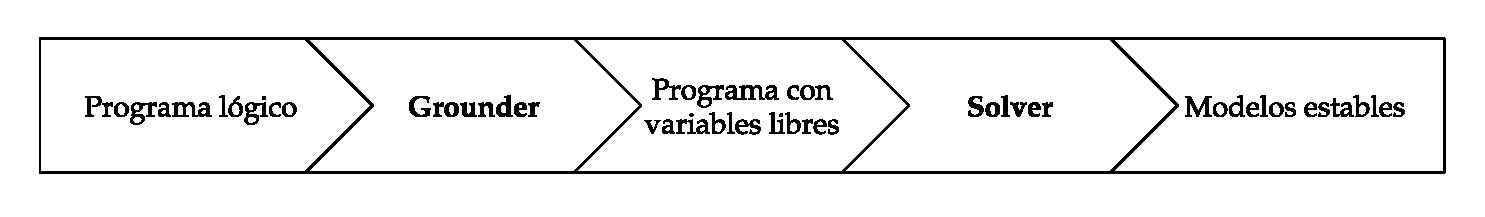
\includegraphics[height=4em]{images/ASP}
	\label{fig:asp}
	\caption{Ejemplo de ejecución de ASP}
\end{figure}

Unas de las herramientas más importantes de ASP son la de Potassco\footnote{http://potassco.org}, la cual son un conjunto de herramientas para ASP desarrolladas en la Universidad de Postdam. Contienen las herramientas fundamentales como un grounder llamado \textit{gringo}; un solver que es \textit{clasp}; y una herramienta que aguntina todo el sistema ASP, \textit{clingo}. Así mismo, añade más funcionalidades al lenguaje ASP, como puede ser al resolución iterativa, debido a que permite embeber otros lenguajes como Lua, el cual está explicado en la Sección \ref{subsec:lua}, o Python, que pueden interactuar con el programa escrito en ASP mediante la interfaz o \textit{API built-in} de clingo. \\

Estas herramientas serán claves a la hora de realizar este proyecto, ya que, como veremos más adelante, debido a la naturaleza de ASP, serán la base sobre la que se construirá todo el proyecto.

\subsection{Lua}\label{subsec:lua}

Lua\footnote{http://www.lua.org} \cite{Ierusalimschy:2016:PLF:3002843} (del portugués Luna), es un lenguaje de programación de propósito general, de scripting y multiparadigma (procedural, orientado a objetos basado en prototipos, funcional y \textit{data-driven}). Fue pensado para ser embebido en cualquier aplicación independientemente de la plataforma sobre la que se ejecuta. Su intérprete esté escrito en ANSI C y contiene una API en C muy simple. \\

Uno de los puntos fuertes de Lua es que permite construir nuevos tipos en base a arrays asociativos, que también permiten extender la semántica del lenguaje al aplicar metadatos a estos. A parte de esto, también facilita la tarea al programador al tener un recolector incremental de basura que se encarga de gestionar automáticamente la memoria. Además, Lua es de tipado dinámico, y se ejecuta sobre un intérprete bytecode en una máquina virtual basada en registros, ejecutándose más rápido que otros lenguajes ejecutados sobre una máquina virtual basada en \textit{stack}, como puede ser Java. \\

A parte de esto, existen otras implementaciones y dialectos basados en Lua, como LuaJIT\footnote{http://luajit.org/luajit.html}, que es una implementación de la máquina virtual de Lua que compilar en tiempo de ejecución y no antes de ejecutarse; y MoonScript\footnote{https://moonscript.org}, un lenguaje de scripting basado en Python que extiende el lenguaje de Lua al añadir orientación a objetos basados en clases, una forma más eficiente de lenguaje funcional y nuevas estructuras y elementos que no contenía Lua. \\

Exiten otras implementaciones que lo único en lo que se diferencian de la implementación estándar es que expanden las funciones básicas o implementan bibliotecas por defecto. A estas implementaciones se llaman \textit{Lua Players} o \textit{Lua Engines}, que principalmente son destinadas para la creación de videojuegos, ya que añaden la implementación de las bibliotecas gráficas para una plataforma concreta, como pueden ser SDL o OpenGL. Los más destacados son los intérpretes no oficiales para consolas de Sony y Nintendo, y los intérpretes para ordenador y móviles como Corona, Cocos-2D, Moai y LÖVE [ver sección \ref{subsec:love2d}]. \\

Como ya expliqué en la Sección \ref{subsec:asp}, las herramientas ASP que se usarán permiten usar este como un lenguaje embebido, lo que nos permitirá controlar la ejecución de la base. Así mismo, tomaremos el \textit{engine} LÖVE para crear una interfaz gráfica para que los usuarios puedan trabajar mejor con la edición de los mapas.

\subsection{JSON}

JSON\footnote{https://www.json.org} (acrónimo de JavaScript Object Notation) es un formato abierto \cite{JSON} ligero de intercambio de información. Está pensado para la transmisión de objetos de datos usando texto en un formato legible por humanos, pudiendo ser leído y modificado fácilmente. \\

A demás, puedes ser fácilmente analizado y generado por máquinas, de ahí que a pesar de que en sus inicios fue pensado como un subconjunto del lenguaje de programación JavaScript/ECMAScript, actualmente es un lenguaje independiente debido a que muchos otros lenguajes incluyen actualmente herramientas para poder leerlo y modificarlo de forma nativa. \\

JSON se basa en dos tipos de estructuras:

\begin{itemize}
	\item Un mapa asociativo que guarda pares (nombre, valor). Esta estructura se reconoce en el estándar como \textit{object}.
	\item Una lista ordenada que guarda valores. Esta estructura se reconoce en el estándar como \textit{array}.
\end{itemize}

Estas estructuras se pueden mezclar independientemente, pudiendo generar listas de objetos u objetos que contienen listas de elementos. \\

Debido estas características, y a que Lua soporta este estándar mediante bibliotecas externas, se usará para el intercambio de datos entre el programa principal y la parte lógica, así como será utilizado para almacenar temporalmente los escenarios antes de ser exportados al software final.

\section{Herramientas}

Aparte de las tecnologías usadas para la construcción del proyecto, se ha usado distintas herramientas que nos han servido a la hora de elaborar y desarrollar el sistema planteado.

\subsection{Atom}

Atom\footnote{https://atom.io} es un editor de texto gratuito y de código abierto basado en Electron, que es un \textit{Framework} para crear aplicaciones nativas con tecnología Web. Está desarrollado por GitHub Inc. e integra dentro de su interfaz la herramienta Git para el control de versiones. Se puede extender las funcionalidades de Atom mediante \textit{plugins} escritos con Node.js, los cuales permiten desde resaltar la sintaxis de un determinado lenguaje de programación, cambiar el tema del editor, hasta añadir terminales, autocompletado de texto o nuevas herramientas para desarrollar/depurar código fuente. Entre estos plugins cabe destacar que para este proyecto podemos encontrar algunos que nos permiten resaltar la sintaxis de Lua y de ASP, así como iniciar LÖVE y ASP desde el propio editor. Debido a estas características, se usará este editor como una de las herramientas principales.

\subsection{Git}

Git\footnote{https://git-scm.com} es un sistema de control de versiones distribuido y de código abierto creado para la gestión de código fuente y desarrollo de software. Fue creado por Linus Trovalds como una alternativa libre y gratuita a BitKeeper para el desarrollo del kernel Linux por la comunidad. Está enfocado en la rapidez y eficiencia al procesar proyectos grandes, la integridad de datos, la seguridad mediante autentificación criptográfica y el fuerte soporte de un flujo de trabajo no lineal y distribuido. \\

Debido a estas características, Git es uno de los sistemas de control de versiones más importantes hoy en día, por lo que ha permitido que existan servicios de alojamiento en linea que incluyen esta herramienta:

\begin{itemize}
	\item GitLab\footnote{https://gitlab.com}, creado por dos programadores ucranianos y que hoy en día es gestionado por GitLab Inc. Es usado por organizaciones como Sony, IBM, NASA, CERN o GNOME Foundation. Permite realizar gratuitamente repositorios privados, gestionar grupos y realizar rastreo de \textit{issues} y funcionalidades de CI/CD.
	\item Phabricator\footnote{https://www.phacility.com}, creado por Facebook como herramienta interna que integra también Mercurial y Subversion. Actualmente es de código abierto y lo usan empresas como Blender, Cisco Systems, Dropbox o KDE.
	\item Bitbucket\footnote{https://bitbucket.org}, creado por Atlassian. Este sistema integra Mercurial desde sus inicios y Git desde 2011, y está pensado para ser integrado con el resto de productos como Atlassian como Jira, Confluence y Bamboo.
	\item GitHub\footnote{https://www.github.com}, creado por tres estudiantes estadounidenses, hoy en día es gestionado por GitHub Inc. empresa que fue adquirida por Microsoft en 2018. Permite realizar rastreo de \textit{bugs}, wikis, gestión de tareas y petición de funcionalidades. Es usado por empresas como Microsoft, Google, Travis CI, Bitnami, DigitalOcean y Unreal Engine. Con la popularidad de GitHub nacieron varios servicios, como el Education Program, que permite a estudiantes el acceso gratuito a herramientas de GitHub y de partners; Gist, que permite usar GitHub como un hosting de \textit{snippets} y GitHub Marketplace, que permite comprar servicios con los que aumentar las funcionalidades en los proyectos y que muchos de ellos son gestionados por partners.
\end{itemize}

\subsection{LÖVE}\label{subsec:love2d}

LÖVE\footnote{https://love2d.org} (o también conocido como Love2D) es un motor de código libre multiplataforma para la creación de juegos en 2D mediante el lenguaje Lua. Está hecho en C++ y añade una API al lenguaje Lua para que el programador pueda usar las bibliotecas OpenGL ES y SDL de una forma muy simplificada mediante funciones y tipos creados en Lua. Con el paso del tiempo también fue incluyendo un motor de físicas 2D o bibliotecas para el manejo de fuentes FreeType, manejo de strings en UTF-8, funciones para usar sockets y una biblioteca especializada en conexión a videojuegos llamada ENet. Así mismo, debido al crecimiento de la comunidad, esta fue creando bibliotecas no oficiales que expanden el funcionamiento del motor, como bibliotecas para añadir interfaces inmediatas, soporte para técnicas usadas en videojuegos, orientación a objetos basada en clases o incluso portar el motor a otras plataformas o lenguajes. \\

Debido a la sencillez para poder dibujar en pantalla, así como poder integrar las bibliotecas gráficas creadas para LÖVE, este motor va a ser una de las herramientas principales que se usarán para la construcción de la interfaz de usuario en este proyecto.